\documentclass[10pt,a4paper]{article}
\usepackage[margin=19mm]{geometry}
\usepackage[T1]{fontenc}
\usepackage{lmodern}
\usepackage{amsmath,amssymb,mathtools}
\usepackage{microtype}
\usepackage{graphicx}
\usepackage[hidelinks]{hyperref}
\setlength{\parindent}{0pt}
\setlength{\parskip}{5pt}
\setlength{\abovedisplayskip}{6pt}
\setlength{\belowdisplayskip}{6pt}
\newcommand{\R}{\mathbb R}
\newcommand{\E}{\mathbb E}
\newcommand{\ip}[2]{\langle #1,#2\rangle}
\newcommand{\norm}[1]{\left\|#1\right\|}
\DeclareMathOperator{\dist}{dist}
\hypersetup{pdftitle={Stochastic FRAMES: nonconvex 1024-dimensional experiment},
 pdfsubject={Problem, randomized initialization, parameter schedules, gap notation, and plots}}

\begin{document}
\begin{center}
{\Large\bfseries Stochastic FRAMES: experiment specification}\\[4pt]
{\large Nonconvex $\ell_1$-constrained least squares in dimension $1024$}\\[3pt]
14 October 2026 \quad $\cdot$ \quad Random negative-vertex initialization
\end{center}

\textbf{Problem.} Let $d=1024$, and let $e_j$ denote the vector with entry $1$ in position $j$
and $0$ elsewhere. The problem is
\[
\boxed{\min_{x\in C} F(x),\qquad F(x)=f(x)+g(Tx).}
\]
The four ingredients are
\begin{align*}
f(x)&=\frac14\bigl(\norm{x-a-b}_2^2+\norm{x-a+b}_2^2\bigr)
       -\frac58(u^\top x)^2
       =\frac12\norm{x-a}_2^2+\frac18-\frac58(u^\top x)^2,\\
C&=\{x\in\R^{1024}:\norm{x}_1\le1\},\qquad T=I_{1024},\\
g(z)&=\iota_D(z)=\begin{cases}0,&z\in D,\\+\infty,&z\notin D,\end{cases}
\qquad D=\R_+^{1024}.
\end{align*}
Thus original feasibility means $x\ge0$ and $\sum_j x_j\le1$. The data vectors are
\[
a_j=\begin{cases}
1/32,&1\le j\le64,\\
-3/128,&65\le j\le128,\\
1/128,&129\le j\le1024,
\end{cases}
\qquad
b_j=\frac{(-1)^{j-1}}{64},
\qquad
u_j=\begin{cases}
(-1)^{j-1}/8,&1\le j\le64,\\
0,&65\le j\le1024.
\end{cases}
\]
With $Q:=I-\frac54uu^\top$, the true smooth gradient is $\nabla f(x)=Qx-a$.
Since $\norm{u}_2=1$, the Hessian $Q$ has eigenvalues $-1/4$ and $1$: the objective is
nonconvex and globally $1$-smooth. Nonconvexity also occurs within the feasible set:
if $x_s$ has its first $64$ entries equal to $1/64$ and all other entries zero, then
\[
x_s+tu\in C\cap D,\qquad F(x_s+tu)=\frac{91}{512}-\frac{t^2}{8},
\qquad |t|\le\frac18.
\]

\textbf{Finite sum and stochastic oracle.} Sample one of two components uniformly:
\[
f_\varepsilon(x)=\frac12\norm{x-a+\varepsilon b}_2^2-\frac58(u^\top x)^2,
\qquad \varepsilon\in\{-1,+1\},\qquad f=\tfrac12(f_{-1}+f_{+1}).
\]
At iteration $k$, draw a fresh independent $\varepsilon_k$ and use
$q_k=\nabla f_{\varepsilon_k}(x_k)=Qx_k-a+\varepsilon_k b$.
Writing $\mathcal F_k$ for the history before this draw (including $x_0$),
\[
\E[q_k\mid\mathcal F_k]=\nabla f(x_k),\qquad
\E[\norm{q_k-\nabla f(x_k)}_2^2\mid\mathcal F_k]=\norm{b}_2^2=\frac14.
\]
This is one sampled least-squares \emph{block} gradient per update, with the common
concave quadratic included.

\textbf{Initialization and run parameters.} For each seed $s\in\{0,\ldots,7\}$, independently
of the oracle draws, sample $J_s$ uniformly from $\{1,\ldots,1024\}$ and set
\[
\boxed{x_0^{(s)}=-e_{J_s}.}
\]
The initial point has one randomly chosen entry equal to $-1$ and all other entries
equal to $0$. It satisfies $\norm{x_0^{(s)}}_1=1$ and $\dist_D(x_0^{(s)})=1$.
The initial momentum estimate is the first sampled gradient: $m_0=q_0$.

The experiment uses $N=32768$ updates per seed, $8$ seeds, and float64 arithmetic.
For $k=0,\ldots,N-1$, the schedules are
\[
\boxed{\gamma_k=(k+1)^{-3/4},\qquad
\beta_k=(k+1)^{-1/4},\qquad
\alpha_k=(k+1)^{-1/2}.}
\]
Here $\gamma_k$ is the Frank--Wolfe step size, $\beta_k$ the smoothing parameter,
and $\alpha_k$ the weight on the new stochastic gradient. All prefactors are $1$;
there is no warm-up or schedule shift.

\newpage
\textbf{Gap and feasibility notation.} Define $(x_k)_-=\min(x_k,0)$ coordinatewise,
and set
\[
z_k:=\nabla f(x_k)=Qx_k-a,\qquad h_k:=z_k+\frac{(x_k)_-}{\beta_k}.
\]
The reported gaps use these exact vectors. Their definitions and explicit formulas are
\begin{align*}
G_k
&:=\max_{v\in C}\ip{h_k}{x_k-v}
 =\boxed{\ip{h_k}{x_k}+\norm{h_k}_\infty},
&&\text{smoothed Frank--Wolfe gap},\\[3pt]
H_k
&:=\max_{v\in C\cap D}\ip{z_k}{x_k-v}
 =\boxed{\ip{z_k}{x_k}+\max\{0,-\min_j z_{k,j}\}},
&&\text{original constrained gap},\\[3pt]
\delta_k
&:=\dist_D(x_k)
 =\boxed{\norm{(x_k)_-}_2},
&&\text{feasibility violation}.
\end{align*}
Since $x_k\in C$, $G_k\ge0$. However, $H_k$ can be negative when $x_k\notin D$;
the original-gap plot therefore reports $|H_k|$. Feasibility and the original gap
are interpreted together.

\textbf{What the plots average.} For $Z_k\in\{G_k,|H_k|,\delta_k\}$, define
\[
\overline Z_N^{(s)}=\frac1N\sum_{k=0}^{N-1}Z_k^{(s)},\qquad
\widehat A_Z(N)=\frac18\sum_{s=0}^{7}\overline Z_N^{(s)}.
\]
Every pre-update iterate $x_0,\ldots,x_{N-1}$ is included. Thin curves are individual
seed averages; the black curve is $\widehat A_Z(N)$; the band is $\pm2$ standard errors
across the eight seed averages (descriptive). The dashed $N^{-1/4}$ line is a slope
guide, not a numerical upper bound.

\medskip
\textbf{Plots.} Eight seeds with random negative-vertex initialization.
\begin{center}
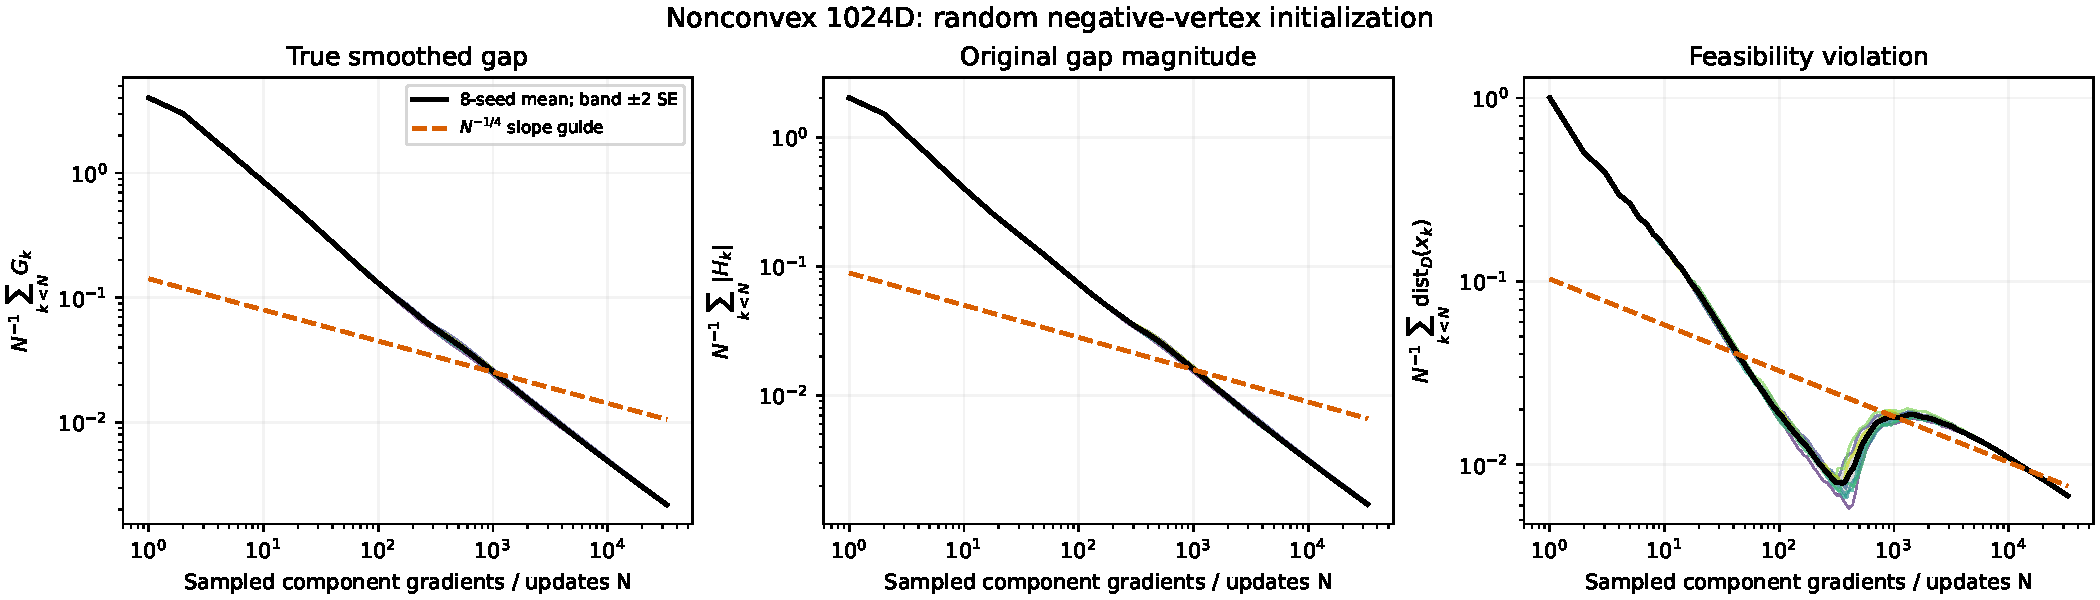
\includegraphics[width=\linewidth]{gaps_feasibility.pdf}
\end{center}
{\small Cumulative averages of $G_k$, $|H_k|$, and $\delta_k$ over all recorded iterates.}

\medskip
\begin{center}
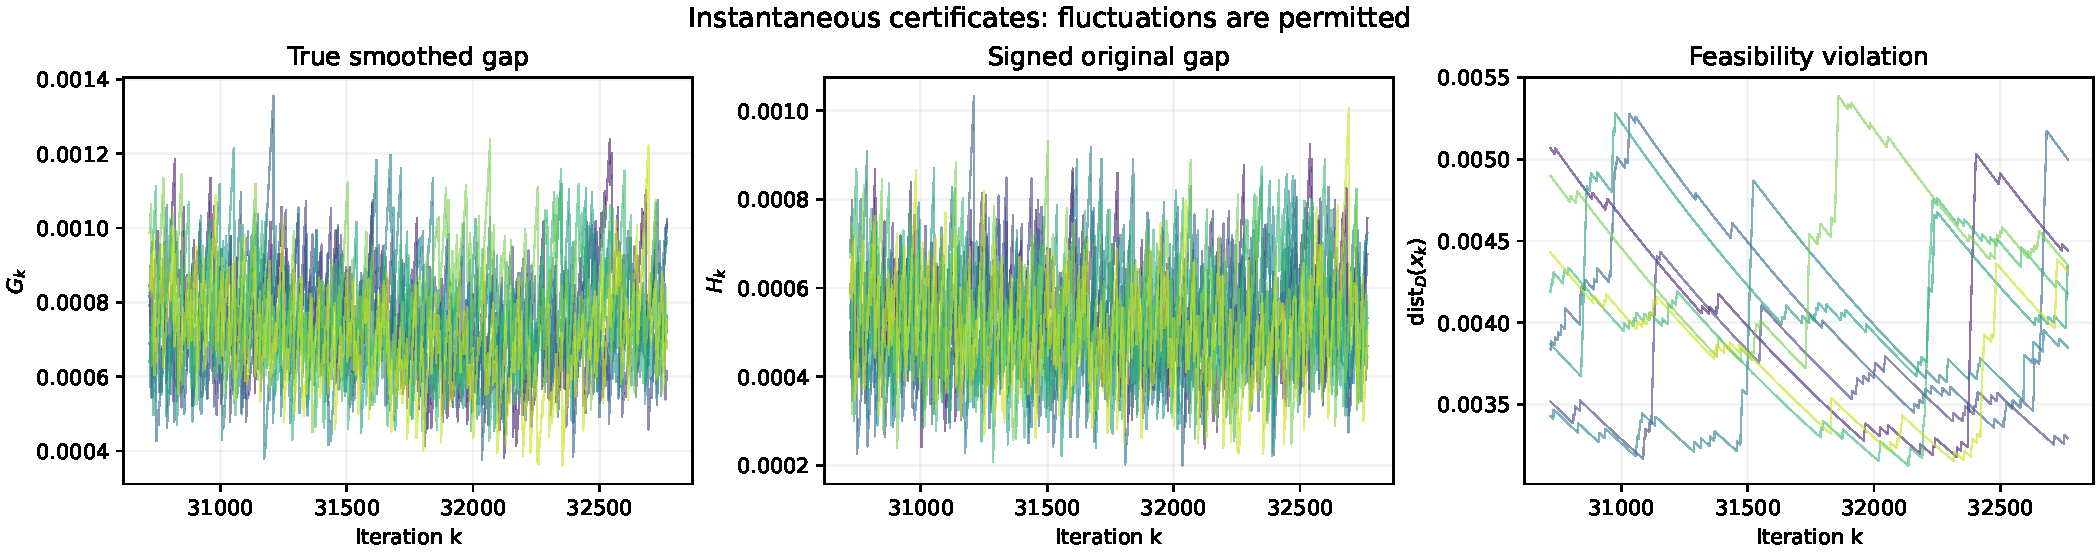
\includegraphics[width=\linewidth]{instantaneous_certificates.pdf}
\end{center}
{\small Individual values of $G_k$, signed $H_k$, and $\delta_k$ during the final $2048$
iterations. Each color represents one seed.}
\end{document}
